\documentclass[journal]{IEEEtran}

\usepackage[utf8]{inputenc}
\usepackage{hyperref}
\usepackage{natbib}
\usepackage{todonotes}
\usepackage{color}
\usepackage{svg}
\usepackage{arrayjob}
\usepackage{multirow}


\hypersetup{
    %bookmarks=true,         % show bookmarks bar?
    unicode=false,          % non-Latin characters in Acrobats bookmarks
    pdftoolbar=true,        % show Acrobats toolbar?
    pdfmenubar=true,        % show Acrobats menu?
    pdffitwindow=false,     % window fit to page when opened
    pdfstartview={FitH},    % fits the width of the page to the window
    pdftitle={TDT4260 - Group 1 - Performance Measurement Unit},    % title
    pdfauthor={Henrik Fegran, Sebastian Bøe, Anders Tvetmarken Akre, Stian Hvatum},     % author
    pdfsubject={Prefetching techniques},   % subject of the document
    pdfcreator={Henrik Fegran, Sebastian Bøe, Anders Tvetmarken Akre, Stian Hvatum},   % creator of the document
    pdfproducer={Henrik Fegran, Sebastian Bøe, Anders Tvetmarken Akre, Stian Hvatum}, % producer of the document
    pdfnewwindow=true,      % links in new window
    colorlinks,       % false: boxed links; true: colored links
    linkcolor=black,          % color of internal links
    citecolor=black,        % color of links to bibliography
    filecolor=magenta,      % color of file links
    urlcolor=cyan           % color of external links
}




\begin{document}

\title{\small{TDT4501 - Toward a SHMAC ISA and Micro Architecture}\\\Huge{An experimental approach on the ARM-ISA}}

\author{Terje~Runde,~MSc.~CS~student~NTNU,
        Stian~Hvatum,~MSc.~CS~student~NTNU}

\maketitle

\begin{abstract}

In order to build more energy efficient traditional hardware, we are in need for
better understanding of how the ISA and its implementation relates to energy
efficiency. This paper investigates the instruction level energy efficiency of
an ARM Cortex-A9, and presents numbers on current drain, pipeline utilization
and other performance data for different instructions. This allows reasoning about
how instructions are executed and how energy efficient their implementation are
in this otherwise publicly closed architecture.

The testbench used in the experiments measures the core current drain by
utilizing a shunt resistor connected directly between the CPU core voltage
supply pins and an external power supply. Measuring isolated core current drain
effectively means skipping other on- and off-chip peripherals as much as possible,
and get a more decent view of what is going on within the processor core. We
also utilize a small and very core-local instruction cache unit called fast-loop-mode,
this together with not using data from memory leaves the caches totally unused.

The results shows that the ARM ISA is well balanced regarding commonly used
instructions, with instructions such as \texttt{add} and \texttt{sub} seemingly
most energy efficient. Unfortunately the ISA suffers from an inefficient handling
of conditional execution and status flags. Both terms cause what is assumed to
be forced synchronization, which again forces inefficient utilization of the
otherwise computationally strong core.

\end{abstract}


\begin{IEEEkeywords}
Hardware prefetching, processor-memory gap, M5 simulator, performance evaluation
\end{IEEEkeywords}

\section{Introduction}

\IEEEPARstart{M}{oore's} law is very often the first word in a paper about computer science.
This is in fact a paper about computer science, and thus starts with the words Moore's law.

\section{Related work}

\section{Description of the ARM Cortex A9 CPU}
The processor we used in the experiment was an ARM Cortex A9 r3p0\footnote{Revision number revealed by printing
the contents of the Main ID Register}, hereby denoted by A9. This processor runs at 1.7GHz,
have 4 32-bit cores, each with its own out-of-order dual issue speculative pipelines\cite{armtech}. The pipeline is split
after the dispatch stage into 4 different lines, each with its own functional units. The different
pipelines is not very well documented, but our experiments together with the common subset of information
found in various documentations\cite{armtech}\cite{7cpu}\cite{lotofdocs}, the four pipelines are structured as follow: Main execution pipeline with a  general ALU,
and a hardware-multiply, secondary execution pipeline with only a general ALU, load-store-pipeline, containing only
an hardware adder to generate addresses, and a floating-point pipeline containing an ordinary FPU and connections to
the NEON unit.

It is a common philosophy that a RISC should consume one clock cycle pr. instruction\cite{unknown}.
For this particular processor made by Advanced RISC Machines, it is not the case. The dual issue and its
 parallell general ALU pipelines enables the processor to achive more than one instruction pr. clock cycle,
and at the same time, it supports multiply, divide and floating point, each taking multiple clock cycle.
It is even so that multiply, divide and floating point takes different amount of cycles according to their
surrounding instructions.

The A9 processor contains an Performance Monitor Unit with 6 generic event counters, a cycle counter
and 58 different events that are mappable to the event counters\cite{armtech}. A list of possible events can be found in
table A.18 in the Cortex-A9 Technical Reference Manual\cite{armtech}.



\section{ISA dependent energy consumption}
% General approach here? Implementation in methodology? Order of appearance?

The need for energy efficient processors is increasing, and in order to achieve
better understanding of how architectural decisions, we propose a method to
measure energy efficiency on the instruction level of a processor.

Our scheme relies on fairly accurate core voltage and power measurements, thus
we have to modify the processor in such a way that core power can be feed
externally.  We run a customized instruction loop, one for each applicable
instruction of the chosen ISA, and measure its power drain.

As each instruction cannot be measured alone, we create an assembly loop that
contains the instruction under test. This loop runs long enough to be measurable
by ordinary laboratory equipment.

Since some instructions takes a different amount of time, the power drain has to be
normalized using statistics gained from performance counters. Applying this
normalization, we can convert point-in-time energy consumption in terms of
wattage to energy per instruction in terms of joules.

As each instruction runs only for a determined amount of time, the measured
instruction loop has to be conditional, thus the list of equal instructions has
to be ended by a conditional branch. The impact of these alien instructions
can be mitigated using statistics and by knowing how the processor works. The
latency introduced by the conditional jump is most likely hidden by the branch
predictor in most modern architectures, either taking a single cycle or hidden
entirely. It has to be noted that its energy consumption is not hidden, and must
be accounted for to get accurate results. This method mainly focuses on
comparison between instructions, and the energy consumption of the condition
calculation and the conditional jump can then be seen as part of the common
baseline.
\todo[inline]{correct assumption?}

When each relevant instruction has been measured, we can compare their
normalized energy consumption and possibly identify patterns where consumption
is greater than expected. This can help in later architectural designs where
energy consumption is important.



\section{Methodology}


\subsection{Test Environment}
\begin{table}
    \begin{tabular}{l|l}
        \hline
        \hline
    Manufacturer	&Hardkernel\\
Platform	&Odroid-X2\\
SoC	&Samsung Exynos 4412 "Prime"\\
CPU Core	&ARM Cortex-A9\\
Number of cores	&4\\
Clock Freq.	&1.7GHz\\
Core voltage	&1.3V\\
OS	&Debian 7 “Wheezy” w/o DVFS\\
Kernel	&3.9 custom\\
        \hline
        \hline
        Voltmeter   &Agilent 34410A\\
        Power supply &Agilent E3631A\\
        Shunt resistor &12m$\Omega$\\
        \hline
        \hline
    \end{tabular}
    \caption{System specifications}
\end{table}
In our experiments, we are using the ODROID-X2 \cite{odroid-x2} developer
platform, which has an Exynos 4412 "Prime" System-on-Chip with four ARM
Cortex-A9 (r3p0) processor cores. We disable three of the cores, leaving only
one core configured to run at a static frequency of $1.7$ GHz.

The Cortex-A9 is a 32-bit out-of-order dual-issue speculative RISC processor,
and even though its primary use is in mobile and embedded applications, it
shares many features with current desktop processors. \cite{patterson}
\cite{hennessy}.

It can issue two instructions per cycle and branches its pipeline to four
functional units, as depicted in \autoref{fig:pipeline}. Most instructions can
execute in either of the two general ALU's, but multiply instructions must
execute in the ALU with a hardware multiplyer. The processor core also has
separate units for floating point operations (the NEON coprocessor) and address
manipulation, but will not be further considered in this paper.

\begin{figure}
    \begin{centering}
        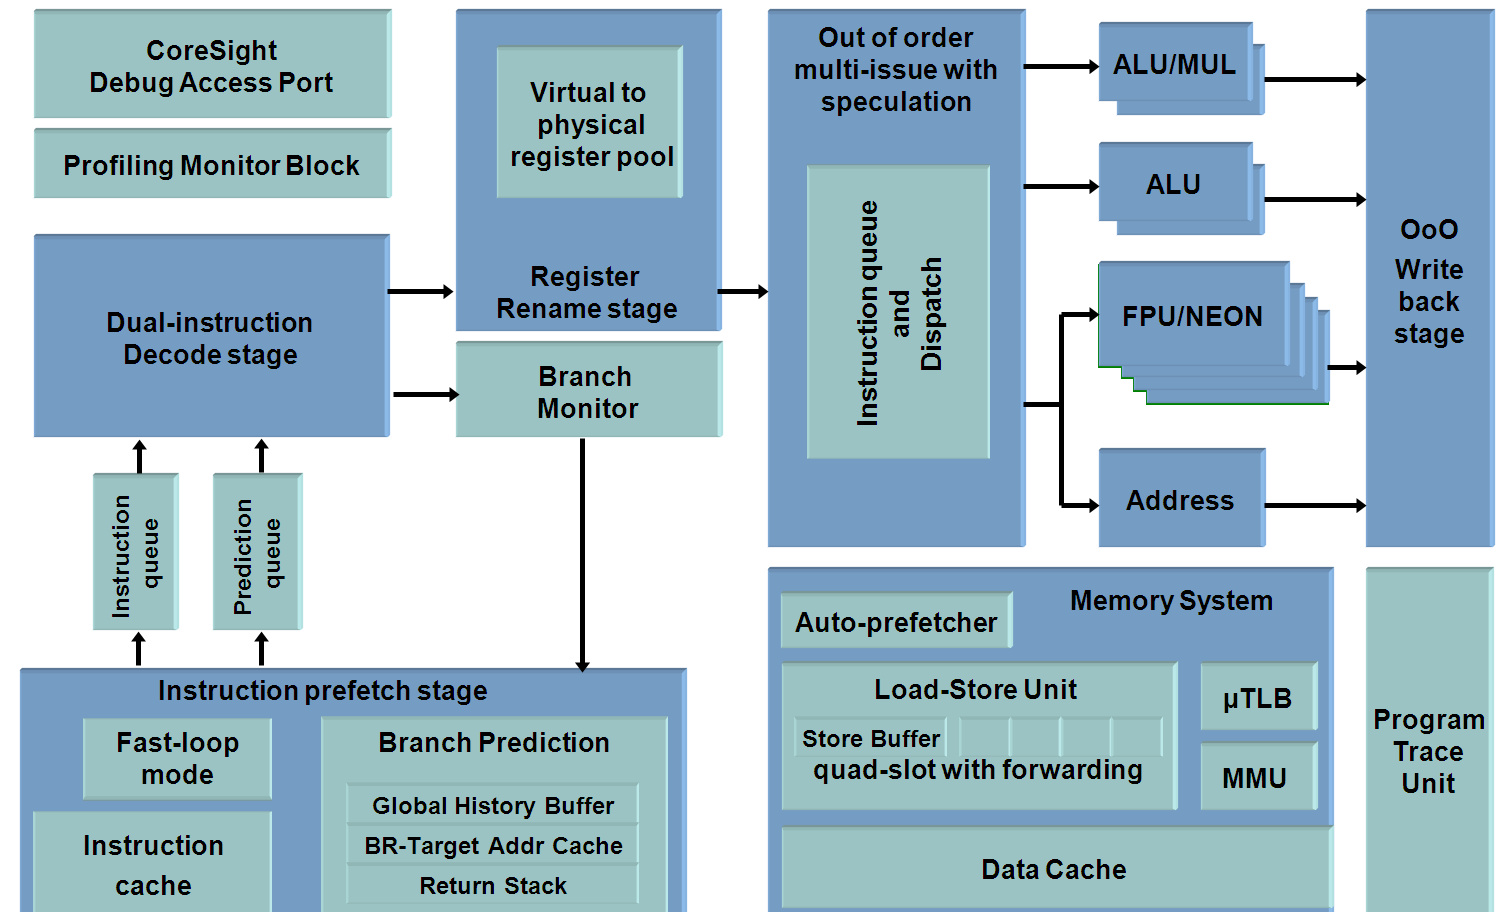
\includegraphics[width=0.48\textwidth]{figures/A9-Pipeline-hres}
        \caption{ARM Cortex-A9 Pipeline and peripherals,\hfill
        figure from ARM Cortex-A9 Whitepaper\cite{a9whitepaper}}
        \label{fig:pipeline}
    \end{centering}
\end{figure}

Because the energy efficiency is often different at different amounts of
workload, we seek to stress the processor as much as possible when we run our
tests. In order to run the processor at it's highest possible throughput, it is
required that we gain some knowledge of it's pipeline and other components
within the CPU. As we are using a proprietary platform as our target
architecture, only some of these details are known. Thus, we define test
programs to stress particular pipeline components and gather statistics using
performance counters. By comparing execution unit counters and the total cycle
count, we obtain detailed (although approximate, due to the speculativity in the
core) information of a test program's execution. \todo[inline]{Elaborate in
detail, see notes/alu-count.txt.}

Official documentation of the internal structure of pipeline stages is limited
to the ``Cortex-A9 Technical Reference Manual'' \cite{armtech} and ``The ARM
Cortex-A9 Processors'' whitepaper \cite{a9whitepaper}. However, by running some
architectural experiments and consulting the performance counters we are able to
infer some details.

\subsection{Architectural Experiments}
\label{arch_experiments}
The A9 processor has 58 distinct events that each can be mapped to one of six
generic event counters in the Performance Monitor Unit (i.e. only six generic
events can be tracked simultaneously). It also has a separate cycle counter. A
complete overview can be seen in table $A.18$ in the Cortex-A9 Technical
Reference Manual \cite{armtech}.

Using performance counters as above, we are able to confirm a feature on the A9
processor that is very vaguely documented; fast-loop\texttrademark mode. As the
name suggests, this feature enables rapid execution of small loops. It does so
by fetching from the instruction cache only at the first loop iteration,
effectively voiding time and energy spent on instruction cache lookups between
iterations. However, which loops that falls into this category is not
documented, but by using performance counters we are able to determine this with
confidence.
\todo[inline]{Add appendix explaining fast-loop microbenchmark.}

Furthermore, executing code within fast-loop limits the number of cache
mispredicts to 2 independently of the iteration count. We confirm this by
looking at the cache mispredict \todo[inline]{name?} performance counter. The
first miss is likely to occur at the end of the first iteration, while the
second occurs on the way out of the loop.

\subsection{Benchmarks}
As a first approximation, the benchmark programs consists of an infinite series
of identical instructions. The A9 core runs at a fixed frequency and we are
providing a fixed core voltage, so energy usage of simple, one-cycle instruction
could be retrieved by running for a fixed time period and applying the following
formula.

\todo[inline]{fix formula}
\begin{equation}
    P_{instruction} = A_{instruction} \cdot V_{core}
\end{equation}
\begin{equation}
    E_{instruction} = P_{instruction} \cdot CPI_{instruction}
\end{equation}


This simple setup does not take the memory system into account; we are
undoubtedly not able to feed the processor instructions at no cost in terms of
access speed and -- more importantly -- memory system energy usage. Thus, we
enhance our setup by running all benchmark code within fast-loop, as explained
above.


\begin{figure}
    \begin{lstlisting}{language=[ARM]Assembler}
    label: instruction
    ... (repeats 13X)
    instruction
    subs
    jne label
    \end{lstlisting}
    \caption{Instruction loop}
    \label{list:inst_loop}
\end{figure}

The technical manual states that branching to immediate locations does not
consume execution unit cycles. Our microbenchmarks branches to immediate
locations, but it does so only when a certain condition is met. We assume that
the calculation of this condition takes normal execution time, but that the
branch is invisible.


\subsection{Power Measurements}
To measure energy consumption, we use an Agilent 34410A
multimeter\cite{agilent34410a} and measures voltage drop over a negligible $12$
$m\Omega$ resistor, set up as shown in \autoref{fig:setup}. The multimeter is
set to sample at full precision at its maximum rate of 1000 Hz. This gives one
sample every 1.7 million instructions with an error of at most 0.002V. It is
obvious that we are unable to observe inter-cycle fluctations, but as we run the
same instruction practically indefinetely we get an average.

We decouple power consumption on the ARM cores and the development board by
modifying the ODROID-X2 and providing a separate power supply for the A9 cores.
They get powered by an external power supply giving $1.3V$ DC, while the rest of
the board is powered from a another power supply at $5.0V$, as depicted in
figure \ref{fig:setup}.

\subsection{Pitfalls}
% temperature, noise (inducted power, etc.), interrupts, memory latency
% (fast-loop)
Since we are comparing the energy efficiency of different instruction in an
asynchronous way, we have to consider factors that affects power usage, as well
as acknowledge that they may differ between runs.

\label{sec:temperature}
One obvious such factor is temperature, both ambient and the chip temperature.
The first may change without our notice, and the second one is determined by the
ambient, the cooling device and what load tasks that was just run on the SoC. On
this specific SoC, Samsung Exynos 4412, we have detected that the difference
from the CPU Thermal Zone 0 being 9$^\circ$ Celsius and 63$^\circ$ Celsius is on
average between 2-4\%. We also detected that some instructions might have as
much as 7\% higher energy consumption when running at the hotter
level\footnote{This was detected with at the {\ttfamily mul}-instruction}. We
have also checked that running a single core at maximum performance over time
does not increase the temperature by more than from idle at 47$^\circ$ Celsius
to 54$^\circ$ Celsius at load. Assuming that it is generally true that a single
core cannot heat the entire SoC with any significant amount, and that the
increase in power consumption is at max 10\% over 50$^\circ$ Celsius, we get

\begin{equation}
    P_{inc} = P_{orig} \cdot T_{inc} \cdot \frac{0.10}{50} = P_{orig} \cdot T_{inc} \cdot 0.002
\end{equation}

Believing that this trend is at least close to linear, output will increase by
0.2\% pr.  degree Celsius increased. Also, we start our measurements at least
half a second after the benchmarks have been started, thus there is plenty of
time for the CPU to gain work temperature. In our tests, the time used to get to
work temperature was humanly instant. Note that we could not log temperature
from on-chip sensors while running our tests, as these sensors are tightly coupled
with DVFS, which is disabled during our benchmarks. The reason for this is that
the modifications done to the chips somehow destroys the communication with the external
power management chip, and thus the development board will not boot with modified
power source together with DVFS modules for Linux.

Another factor that is not that obvious, but at least equally important, is
power inducted in the measurement circuit. Since wires are often winded up on
the test bench, and lab equipment might contain large metal cores with a great
amount of power running through them, unexpected power might be introduced.

We are running Linux on the chip under test, this gives us a much simpler way of
programming the processor to run our tests. The fact that we run an entire
operating system beneath our benchmark programs implies that there is much going
on that we have no direct controls over.  In order to mitigate the artifacts
originating from the operating system, we disable all the mask cable interrupts.

As explained in section \ref{arch_experiments}, we utilize the fast-loop mode of
the processor to mitigate memory access latency. We disable the L1 cache to
easier detect when we are outside the fast-loop mode, and thus we are certain
that there is no memory access going on.

\section{Results}

%\begin{figure*}
%    \centering
%    \includegraphics[width=1.1\textwidth]{figures/graph_0123_base_lowpower_mul-0c6}
%    \label{fig:allmul}
%\end{figure*}
%
%\begin{figure*}
%    \centering
%    \includegraphics[width=0.7\textwidth]{figures/graph_0123_base_mul-0c7}
%    \label{fig:allmul}
%\end{figure*}
%
%
%
%\begin{figure*}
%    \centering
%    \subfloat[][Multiply]
%    {
%        \includegraphics[width=0.49\textwidth]{figures/graph_123_base_mul-0c5}
%        \label{fig:somemul}
%    }
%    \subfloat[][Single Cycle]
%    {
%        \includegraphics[width=0.49\textwidth]{figures/graph_1_base_arith_data_logic-0c5}
%        \label{fig:singlecycle}
%    }
%    \caption{test}
%\end{figure*}

\begin{figure*}[ht]
    \centering
    \includegraphics[width=\textwidth]{figures/graph_01_base_arith_saturate_data_pack_logic-0c6}
    \caption{Energy profile of single-cycle instructions, excluding multiply.}
    \label{fig:singlecycle}
\end{figure*}


\subsection{Introduction}
In this section we present data gathered from our experiments on the ARM
Cortex-A9.

We distinguish between single-cycle instructions and multi-cycle instructions
because they behave differently in and around the execution pipeline.
Instructions consuming only one cycle are fairly easy to reason about as there
is no need to normalize energy consumption with respect to the cycle count (i.e.
time). However, it is important to also recognize CPU capabilities such as dual
issuing that we have on our processor: All single-cycle ALU instructions execute
pairwise in parallel (one in each ALU), giving a peak performance of two
instructions per CPU cycle. On the other hand, multi-cycle instructions needs to
be carefully considered. Typically, multi-cycle instructions divide work which
can be done only in a subset of the available CPUs (e.g. one) over several
<<<<<<< Updated upstream
cycles, lowering the average current draw. They consume less energy per
time step, but also do less useful work. For all these reasons, we partition the
measured data in two data sets; one for single-cycle instructions and one for
multi-cycle instructions.
=======
cycles, lowering the average current draw. They consume less energy per time
step, but also do less useful work.
>>>>>>> Stashed changes

Observational errors are accounted for by running the power measurement loop
many times for each instruction. We also sleep 30 seconds in between
instructions to diminish the effect of temperature variations. Running over all
tested instructions typically takes 3 hours and we average the medians for each
instruction run to get a single value.

In the graphs, all bars colored green means that the tested instruction is a
single-cycle instruction, the light blue is two-cycles, and dark blue is
three-cycle instructions. The red bar is the baseline for power measurement.
This baseline is an alias for the least power-consuming instruction we could
find, which is the {\ttfamily setend}-instruction. This instruction sets the
endianness regarding memory operations to eiter big or little
endian \cite{armcompilerref} and setting it to the same endian repeatedly would
resemble constant halting on our processor.

The results presented in the graphs are enumerated as Ampere
$\cdot$ cycles, which means that instructions using more time is normalized by
adding up their power drain with the time used in the pipeline. The results are
not converted into watts, joule or anything else that would be more convenient
in order to state a number on each instructions energy consumption. This is
because this paper investigates how each instruction differs from other
instructions in the same ISA, and thus we look at the power drain at the
processor core when a given instruction resides within it, multiplied by the
number of cycles the instruction consumes. 

During measurements, the core voltage was keept stable at
$1.3V\pm50mV$ during testing. The measurements where done with as full
pipelines as possible, avoiding hazards and instruction loading as much as
possible. This means that instructions that utilize more parts of the processor
will most likely be more energy consuming than those using only few components.
This is also shown with our {\ttfamily baseline}-measurement, as we assume that
the {\ttfamily setend}-instruction merly changes some status flags.



%Some instructions use variable amount of time. This section will contain
%information about how we normalize and compare energy consumption of
%these instructions. It will be difficult to compare single cycle instructions
%to the multi cycle ones, as the single cycle instructions is often the ones
%utilizing more than one ALU at a time. Also, the multi-cycle ones will most
%likely pipeline up very differently than the single cycle ones. We will try to
%draw a conclusion about the results, but it is important to note the differences
%in the execution path of these two categories.

\subsection{Single-Cycle Instructions}
On our target CPU, 70 of the 116 tested instructions\footnote{118 including conditionals} consumes a single cycle,
while the remaining 46 uses 2 or 3.

\begin{figure}
    \centering
    \includegraphics[width=0.4\textwidth]{figures/graph_01_base_cond-0c6}
    \caption{Energy profile showing conditional execution.}
    \label{fig:cond}
\end{figure}

The results in \autoref{fig:singlecycle} shows that the ordinary single-cycle instructions
does not differ very much. Instructions like {\ttfamily rev} and {\ttfamily sel} are on the
top, which can be explained by looking on how these instructions move nearly all bits in
the operands around, while {\ttfamily cmp} and the different shift-instructios are most likely
moving fewer bits around. A more interesting result is how instructions bearing the {\ttfamily s}-flag
seems to have a lover consumption than their non-{\ttfamily s}-companion. It is hard to reason about
such, since we do not have access to the inner workings of this processor.

The results from the conditional-execution scheme brought by this ISA are also an interesting matter. We
can see from \autoref{fig:cond} how different versions of {\ttfamily add} compares. In the figured test,
{\ttfamily addne} is committed every time, while {\ttfamily addeq} never has its results committed. It is
interesting to see that even though {\ttfamily addeq} is never committed, it uses almost as much power as
the other {\ttfamily add}s. We can assume that with the addition of out-of-order scheduling, conditional
execution might be harder to implement.

\autoref{fig:singlecycle} shows that the {\ttfamily nop}-instruction has a rather low power consumption. This
is a bit missguiding, as the {\ttfamily nop}-instruction is actually a {\ttfamily mov r0,r0}-instruction, and thus
has both a read-after-write and a write-after-write hazard on it self. This makes the {\ttfamily nop}-instruction
serialize it self, and it is hard to fill the pipeline with this instruction. With this in mind, it makes sense
that {\ttfamily nop} works in this way, as it is often used to fill out clock cycles with non-destructive work. It
would not make sense to optimize the {\ttfamily nop} instruction, as it would merly fail to complete it's goal as
a space-and-time filler.

\begin{figure*}
    \centering
    \includegraphics[width=\textwidth]{figures/graph_0123_base_mul-0c6}
    \caption{Energy profile of multiply instructions.}
    \label{fig:allmul}
\end{figure*}

\begin{figure}
    \centering
    \includegraphics[width=0.48\textwidth]{figures/graph_023_base_quad_saturate_extend-0c6}
    \caption{Energy profile of multi-cycle instructions, excluding multiply.}
    \label{fig:multicycle}
\end{figure}


\subsection{Multi-Cycle Instructions}

%See \autoref{fig:multicycle} and \autoref{fig:allmul}
%\begin{itemize}
%    \item The difference between instructions are much larger in the multi-cycle
%        graphs.
%    \item Talk about mul, and why it might differ that much (especially 2 and 3 cycle ones)
%\end{itemize}

46 of the instructions that was compared used more than 1 cycle to complete their results, 


\subsection{Evaluation}
\begin{figure}
    \centering
    \includegraphics[width=0.48\textwidth]{figures/heat}
    \caption{Changes in heat and energy consumption for {\ttfamily add} at different runs together with heatsink and ambient temperature}
    \label{fig:heat}
\end{figure}

Each instruction was measured 41 times. For each run, there was small changes in
power consumption, but the relation trends was equal for every run.
As stated in \autoref{sec:temperature}, the power consumption is not easily pushed by temperature. \autoref{fig:heat} shows how the change in power consumption of the instruction
{\ttfamily add} over different runs combined with the ambient temperature the
heatsink temperature. According to these results, we assume that the change in
power consumption was not due to heat. We did not log heat for all test runs,
but assume that the results from \autoref{fig:heat} holds, and that this small
change in heat is not responsible for any disturbance in the power consumption
measurements.



\section{Discussion}


\section{Conclusion}
This is where we will put the conclusion

\subsection{Further Work}

We have not yet dived into how instruction operands affects the energy usage on
modern processors. We would think that instruction patterns that causes a high
degree of bit toggling would yield higher energy usage, due to the amount of
TODO. However, writing valid benchmarks stressing these pattern is difficult on
modern architectures because of the out-of-order non-determinism.

FPU instructions
\todo[inline]{Please write.}

\bibliographystyle{plain}
\bibliography{./bibliography}

\end{document}
